\documentclass{beamer}
\usepackage[utf8]{inputenc}

\usetheme{Madrid}
\usecolortheme{default}
\usepackage{amsmath,amssymb,amsfonts,amsthm}
\usepackage{txfonts}
\usepackage{tkz-euclide}
\usepackage{listings}
\usepackage{adjustbox}
\usepackage{array}
\usepackage{tabularx}
\usepackage{gvv}
\usepackage{lmodern}
\usepackage{circuitikz}
\usepackage{tikz}
\usepackage{graphicx}

\setbeamertemplate{page number in head/foot}[totalframenumber]

\usepackage{tcolorbox}
\tcbuselibrary{minted,breakable,xparse,skins}



\definecolor{bg}{gray}{0.95}
\DeclareTCBListing{mintedbox}{O{}m!O{}}{%
  breakable=true,
  listing engine=minted,
  listing only,
  minted language=#2,
  minted style=default,
  minted options={%
    linenos,
    gobble=0,
    breaklines=true,
    breakafter=,,
    fontsize=\small,
    numbersep=8pt,
    #1},
  boxsep=0pt,
  left skip=0pt,
  right skip=0pt,
  left=25pt,
  right=0pt,
  top=3pt,
  bottom=3pt,
  arc=5pt,
  leftrule=0pt,
  rightrule=0pt,
  bottomrule=2pt,
  toprule=2pt,
  colback=bg,
  colframe=orange!70,
  enhanced,
  overlay={%
    \begin{tcbclipinterior}
    \fill[orange!20!white] (frame.south west) rectangle ([xshift=20pt]frame.north west);
    \end{tcbclipinterior}},
  #3,
}
\lstset{
    language=C,
    basicstyle=\ttfamily\small,
    keywordstyle=\color{blue},
    stringstyle=\color{orange},
    commentstyle=\color{green!60!black},
    numbers=left,
    numberstyle=\tiny\color{gray},
    breaklines=true,
    showstringspaces=false,
}
\begin{document}

\title 
{1.4.18}
\date{September 1,2025}


\author 
{ADHARVAN KSHATHRIYA BOMMAGANI -EE25BTECH11003}






\frame{\titlepage}
\begin{frame}{Question}
Show that $\vec{P}$(5,-3) is the point of trisection of the line segment that join the points  $\vec{A}$ (7,-2) and  $\vec{B}$ (1,-5).
\end{frame}

\begin{frame}{formula}
 \textbf{D} divides $BC$ in the ratio $k : 1$, 
\begin{align}
        \vec{D} = \frac{k\vec{C} + \vec{B}}{k + 1}
\end{align}
\end{frame}


\begin{frame}{Theoretical Solution}
\begin{align}
\text{Let } 
\vec{A} = \myvec{ 7 \\ -2 },
\vec{B} = \myvec{ 1 \\ -5 }
\end{align}


\textbf{Point  $\vec{P}$  (Further to  $\vec{A}$ , Ratio 2 : 1):}
\begin{align}
    \vec{P}=\begin{myvec}{\vec{A}& \vec{B}}\end{myvec}\begin{myvec}
        {\frac{2}{3}\\\frac{1}{3}}\end{myvec}    
\end{align}
\begin{align}
\implies \vec{P}=\begin{myvec}{ 7 & 1\\ -2 & -5 }\end{myvec}\begin{myvec}
        {\frac{2}{3}\\\frac{1}{3}}\end{myvec}\\
\end{align}


\begin{align}
\vec{P} = \begin{myvec}{
\frac{1 \times 1 + 2 \times 7}{3} \\
\frac{1 \times -5 + 2 \times (-2)}{3}
}\end{myvec}
= \begin{myvec}{ 5 \\ -3 }\end{myvec}
\end{align}
\end{frame}

\begin{frame}
\textbf{Point \( \vec{Q} \) (Nearer from \( \vec{A} \), Ratio 1 : 2):}
\begin{align}   
\vec{Q} = \begin{myvec}{\vec{A}& \vec{B}}\end{myvec}\begin{myvec}
        {\frac{1}{3}\\\frac{2}{3}}\end{myvec}    
\end{align}       

\begin{align}
\implies \vec{Q}=\begin{myvec}{ 7 & 1\\ -2 & -5 }\end{myvec}\begin{myvec}
        {\frac{1}{3}\\\frac{2}{3}}\end{myvec}\\
\end{align}


\begin{align}
\vec{Q} = \begin{myvec}{
\frac{2 \times 1 + 1 \times 7}{3} \\
\frac{2 \times (-5) + 1 \times (-2)}{3}
}\end{myvec}= \begin{myvec}{ 3 \\ -4 }\end{myvec}
\end{align}

\begin{align}
\vec{P}=\myvec{5\\-3}\ \  \vec{Q}=\myvec{3\\-4}
\end{align}    
\end{frame}

\begin{frame}
    \vspace{5em}
\textbf{Graph of the line segment AB with trisection points P and Q}
\begin{figure}[H]
    \centering
    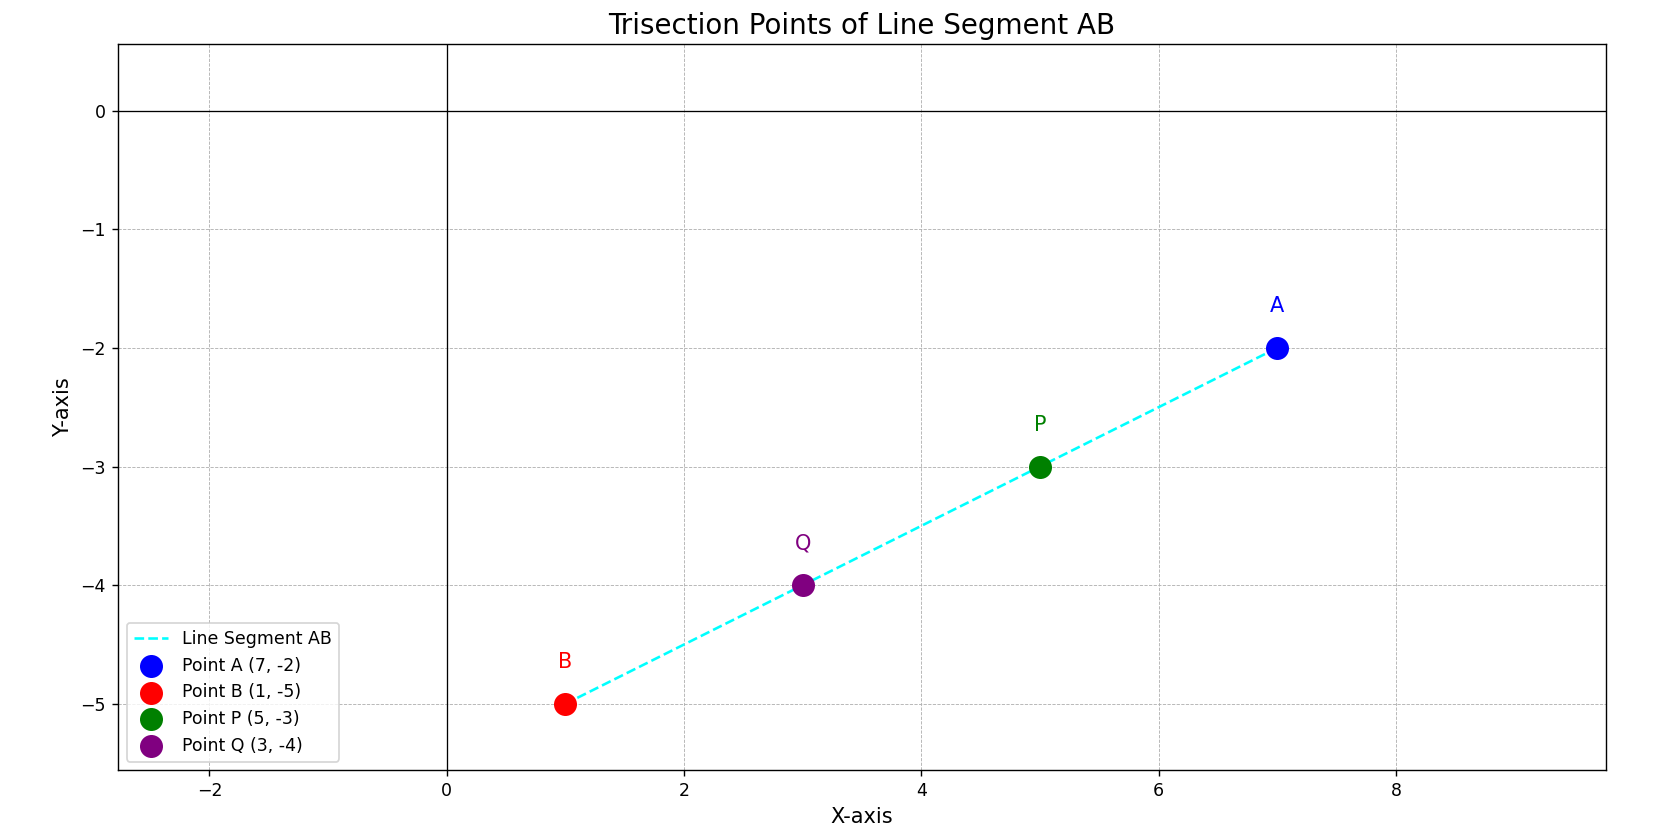
\includegraphics[width=0.75\columnwidth]{figs/fig1.png}
    \caption{Figure for 1.4.18}
    \label{fig1}
\end{figure}
\end{frame}

\end{document}